%%%%%%%%%%%%%%%%%%%%%%%%%%%%%%%%%%%%%%%%%
% Minimalist Book Title Page 
% LaTeX Template
% Version 1.0 (27/12/12)
%
% This template has been downloaded from:
% http://www.LaTeXTemplates.com
%
% Original author:
% Peter Wilson (herries.press@earthlink.net)
%
% License:
% CC BY-NC-SA 3.0 (http://creativecommons.org/licenses/by-nc-sa/3.0/)
% 
% Instructions for using this template:
% This title page compiles as is. If you wish to include this title page in 
% another document, you will need to copy everything before 
% \begin{document} into the preamble of your document. The title page is
% then included using \titleTH within your document.
%
%%%%%%%%%%%%%%%%%%%%%%%%%%%%%%%%%%%%%%%%%

%-------------------------------------------------------------------------------------
%	PACKAGES AND OTHER DOCUMENT CONFIGURATIONS
%-------------------------------------------------------------------------------------

\documentclass[11pt]{article} %extarticle
\usepackage[utf8]{inputenc} 
\usepackage[T1]{fontenc}
\usepackage[french,UKenglish]{babel}
\usepackage{graphicx}%images
\usepackage[svgnames]{xcolor} % Required to specify font color
\usepackage[babel=true]{csquotes}
\usepackage{mathpazo}
\usepackage{floatrow}
\usepackage{geometry}%réglages mise en page
\geometry{%
a4paper, % note : l'option a4paper tuait la marge supérieure.
body={170mm,230mm}, %
left=25mm,top=25mm,right=25mm, %
headheight=21mm,headsep=7mm,
marginparsep=4mm,
marginparwidth=20mm, %
footnotesep=50mm
}
\usepackage{mdframed} %to use simple box
%\usepackage{framed}
\usepackage{layout}

\title{Project2}

\newcommand*{\poo}{\fbox{INFO-F-405}} % Generic publisher logo
\newcommand{\gate}[1]{\includegraphics[height=3ex]{Gates/#1.png}}
%-------------------------------------------------------------------------------------
%	TITLE PAGE
%-------------------------------------------------------------------------------------

\newcommand*{\titleTH}{\begingroup % Create the command for including the title page in the document
\raggedleft % Right-align all text
\vspace*{\baselineskip} % Whitespace at the top of the page
{\LARGE \bsc{Group 1}}\\[0.02\textheight] % Group
{\Large \bsc{Anthony Debruyn}}\\[0.01\textheight] % Author name
{\Large \bsc{Brian Delhaisse}}\\[0.01\textheight] % Author name
{\Large \bsc{Alexis Lefebvre}}\\[0.01\textheight] % Author name
{\Large \bsc{Aurélien Plisnier}}\\[0.167\textheight] % Author name

{\LARGE\bfseries Computer Security }\\[\baselineskip] % First part of the title, if it is unimportant consider making the font size smaller to accentuate the main title

{\textcolor{Red}{\Huge Project 2}}\\[\baselineskip] % Main title which draws the focus of the reader

{\Large \textit{Services and Authentification}}\par % Tagline or further description

\vfill % Whitespace between the title block and the publisher

\vspace*{15\baselineskip}

{\large Prof. \bsc{Olivier Markowitch and Naïm Qachri} \poo}\par % Publisher and logo
\vspace*{3\baselineskip}
{\large \textsc{\today}}\par

\vspace*{1\baselineskip} % Whitespace at the bottom of the page
\endgroup}

% we can also use "framed" instead of "mdframed" (it depends if we want to allow page break or not)
\newcounter{idDesc}
\setcounter{idDesc}{0}
\newcommand{\idDesc}[1]{%
\addtocounter{idDesc}{1}%
\begin{mdframed}
	%\vspace{-0.3cm}
	\begin{description}
		\item[ID:] \arabic{idDesc}
		\item[Description:] #1
	\end{description}
    %\vspace{-0.3cm}
\end{mdframed}
}

\newcounter{idDescName}
\setcounter{idDescName}{0}
\newcommand{\idDescName}[2]{%
\addtocounter{idDescName}{1}%
\begin{mdframed}
	%\vspace{-0.3cm}
	\begin{description}
		\item[ID:] \arabic{idDescName}
        \item[Name:] #1
		\item[Description:] #2
	\end{description}
    %\vspace{-0.3cm}
\end{mdframed}
}

\newcounter{idDescNameTrust}
\setcounter{idDescNameTrust}{0}
\newcommand{\idDescNameTrust}[3]{%
\addtocounter{idDescNameTrust}{1}%
\begin{mdframed}
	%\vspace{-0.3cm}
	\begin{description}
		\item[ID:] \arabic{idDescNameTrust}
        \item[Name:] #1
		\item[Description:] #2
        \item[Level of Trust:] #3
	\end{description}
    %\vspace{-0.3cm}
\end{mdframed}
}

\newcounter{threat}
\setcounter{threat}{0}
\newcommand{\threat}[6]{%
\addtocounter{threat}{1}%
\begin{mdframed}
	%\vspace{-0.3cm}
	\begin{description}
		\item[ID:] \arabic{threat}
        \item[Name:] #1
		\item[Description:] #2
        \item[STRIDE classification:] \textcolor{red}{#3}
        %\item[Known mitigation:] #4
        %\item[Investigation notes:] #5
        \item[Entry points:] #4
        \item[Assets:] #5
       	\item[Threat tree:] #6
	\end{description}
    %\vspace{-0.3cm}
\end{mdframed}
}


%-------------------------------------------------------------------------------------
%	BLANK DOCUMENT
%-------------------------------------------------------------------------------------
% ' “

\begin{document} 

%\pagestyle{empty} % Removes page numbers

\titleTH % This command includes the title page
\thispagestyle{empty}
\clearpage

\section{Threat modeling}
\setcounter{page}{1}

\subsection{Information document}
\begin{mdframed}
	\begin{description}
		\item[Step of the development:] Version 1.0
		\item[Director:] Naïm Qachri
		\item[Participants:] Anthony Debruyn, Brian Delhaisse, Alexis Lefebvre and Aurélien Plisnier.
		\item[Reviewer:] Naïm Qachri
		\item[Location:] ULB
		\item[Description:] Two web services are proposed: a blackboard and a keychain service. The authentification of the web services and the clients is realized by an authentification server. A small website will be made to allow an admin to manage the stored data, and the clients who can have access to those web services.
	\end{description}
\end{mdframed}


\subsection{Use Scenarios}
\idDesc{The services will be accessible from anywhere and only for authorized clients. There are two services: a secure virtual blackboard on which authorized clients can publish posts and  a virtual keychain server in which authorized clients can securely store their passwords.}
\idDesc{An admin will be able to manage the authorized users and their RSA certificate list via a website.}

\subsection{External Dependencies}
\setcounter{idDesc}{0}
\idDesc{The security of the application depends on the AES and RSA keys generator used.}
\idDesc{The security of the application depends on the quality of the certificates generated by OpenSSL.}

\subsection{Implementation Assumptions}
\setcounter{idDesc}{0}
\idDesc{The servers and clients are all aware of the communication protocol used in this project and behave accordingly.}

\subsection{External security notes}
\setcounter{idDesc}{0}
\idDesc{The user is responsible for the strength of his password, the server doesn't have an integrated strength enforcement system that tells the user whether his password is strong enough or not.}

\subsection{Internal security notes}
\setcounter{idDesc}{0}
\idDesc{We trust the implementations of the encryptions and decryptions used in this project, but we read the javadoc associated to understand them.}

\subsection{Levels of trust}
\idDescName{The identity of the web server process.}{This identity is used to authenticate a web server in its database when it stores and retrieves information.}
\idDescName{A registered user.}{The user uses his ID and certificate to authenticate and access the web services.}
\idDescName{The admin.}{The admin uses his PHP application to manage the authorisation server's database.}

\subsection{Assets}
\idDescNameTrust{User's data.}{The user ID and certificate.}{A user with verified token access (2), the admin (3).}

\newpage
\section{Analysis of the model}
\subsection{Data flow diagrams}
\begin{figure}[H]
	\center
    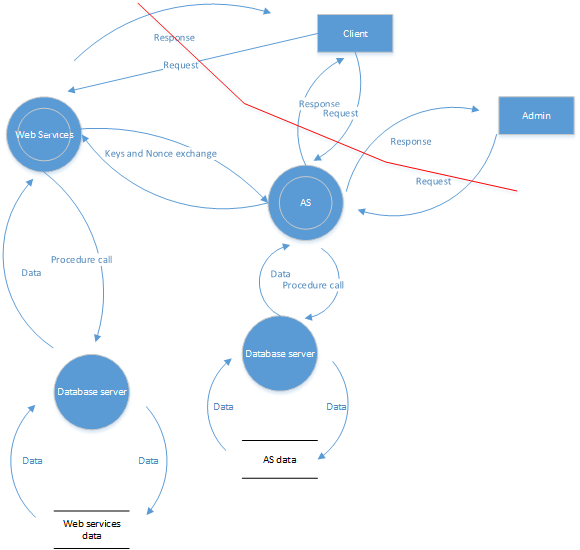
\includegraphics[scale=0.9]{DataFlowDiagram.png}
    \caption{data flow diagram}
    \label{DataFlowDiagram}
\end{figure}

\subsection{Documentation of the potential threats}
%\begin{itemize}
%    \item interception of an encrypted plaintext + attempt to decrypt this one by cyclic-attack (RSA), if the plaintext is the symmetric key --> aie...
%    \item SQL injection for the web service
%    \item attack with a quantum computer (Shor's algorithm)...
%\end{itemize}

%STRIDE:
%1) Spoofing: In the context of network security, a spoofing attack is a situation in which one person or program successfully masquerades as another by falsifying data and thereby gaining an illegitimate advantage.
% http://minsky.gsi.dit.upm.es/semanticwiki/index.php/Principal_Spoofing
%2) Tampering: falsification
%3) Repudiation: A repudiation attack happens when an application or system does not adopt controls to properly track and log users' actions, thus permitting malicious manipulation or forging the identification of new actions. This attack can be used to change the authoring information of actions executed by a malicious user in order to log wrong data to log files.
% http://minsky.gsi.dit.upm.es/semanticwiki/index.php/Repudiation_Attack
%4) Information Disclosure.
%5) Denial of Service.
%6) Elevation of privilege.

% List of attacks:
%http://minsky.gsi.dit.upm.es/semanticwiki/index.php/List_attacks
\threat{Denial of service attack.} %Name
{Many requests are being sent by the attacker(s) to the server in order to saturate/overload this one.} %Description
{D (Denial of Service)} %STRIDE classification
{The listening port of the web server.} %Entry points
{None} %Assets
{see fig. ~\ref{TT1}} %Threat tree

\threat{Gain the client's privileges}
{The attacker acquires a private key and the ID from a valid user (client).}
{E (Elevation of privilege.)}
{}
{User's data.}
{see fig. ~\ref{TT2}}

\threat{Gain the admin privileges}
{The attacker acquires the admin's password.}
{E (Elevation of privilege).}
{Admin}
{Admin's password}
{see fig. ~\ref{TT3}}

\subsection{Threat trees}
\begin{figure}[H]
	\center
    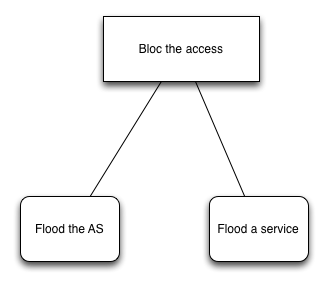
\includegraphics[scale=0.5]{TT1.png}
    \caption{Threat tree}
    \label{TT1}
\end{figure}

\begin{figure}[H]
	\center
    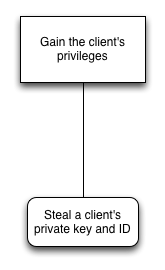
\includegraphics[scale=0.5]{TT2.png}
    \caption{Threat tree}
    \label{TT2}
\end{figure}

\begin{figure}[H]
	\center
    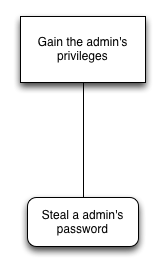
\includegraphics[scale=0.5]{TT3.png}
    \caption{Threat tree}
    \label{TT3}
\end{figure}

%\section{Documentation/validation of the vulnerabilities}

\section{Implementation}
%need to talk about OpenSSL (certificates,...), Needham-Schroeder algorithm,...
%The choices of our implementation must be based on our threat modeling...
\subsection{Web Interface for the admin}
A simple web interface allowing the admin to access and update the authorisation service database was made. It is accessed using https. The https connection was set up using the instruction given during the last practicals.\\ 
The data stored in the AS database was not encrypted due to severe lack of time.
As a proof that the https connection was set up in time, a printscreen of our web app was taken on Linux and added into the directory PHP.

\begin{figure}[H]
	\center
    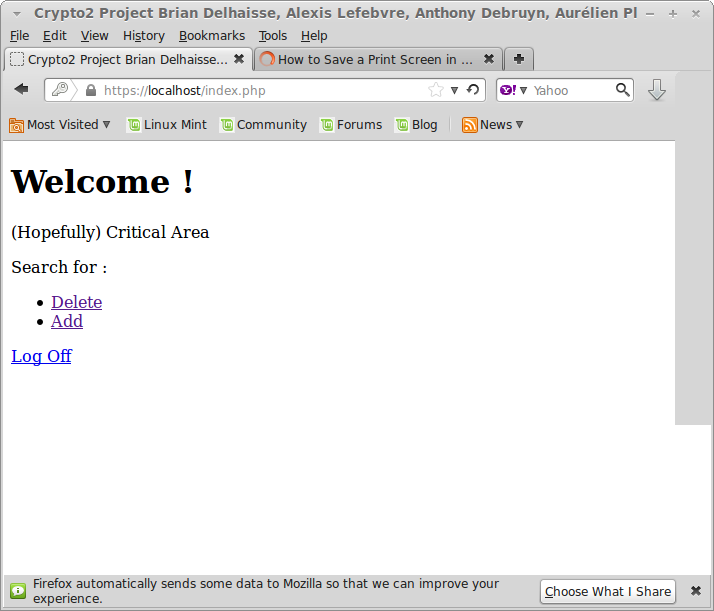
\includegraphics[scale=0.5]{WebApp.png}
    \caption{The web interface for the admin}
    \label{WebApp}
\end{figure}

Here is a short overview of the php files:\\
\begin{description}
	\item[add.php :]Presents a form allowing the admin to type in a user ID and the related certificate to add.
	\item[computeAddUser.php :]Runs a SQL statement to insert the new entry if the typed ID does not already exists in the database or to update the existing user if the ID already exists in the database.
	\item[computeDelete.php :]Runs a SQL statement to delete the entry corresponding to the specified ID.
	\item[footer.php :]A useless footer.
	\item[head.php :]A useless header.
	\item[identityTest.php :]Tests the password typed in by the admin in the logOn page.
	\item[index.php :]Main page of the application, presents the welcome message and the options.
	\item[logOff.php :] Log off.
	\item[logOn.php :] Log on by typing in the password (chicken).
	\item[menu.php :] Contains the options: add, delete, logon and logoff.
\end{description}


\subsection{Authorization Server}
The role of the authorization server is described in the assignments.\\
Here is a short overview of the different classes:\\ 

\begin{description}
\item[Main :] Creates a link to the MySQL database and launches the authorization server.

\item[connection.AuthorisationServer :] The AS server: accepts new connections in a while(true) loop. This class is also able to transmit the AES session key shared by a client and a web service to the web service.

\item[connection.RSASecuredService :] Thread created every time a client contacts the AS. The thread handles the mutual authentication by sending the AS certificate to the client and by implementing the Needham-Schroeder protocol. \\
Once the authentication made, the thread generates and distributes AES session keys. These keys have a cryptoperiod of 2 hours and should be usable only during one session. If a session exceeds 2 hours time, new session keys should be generated. This was not fully implemented due to severe lack of time.

\item[crypto.RsaKey :] This class loads the AS private key and the admin certificate using OpenSSL generated files. The AS certificate is also loaded from the database. \\
A copy of the admin's certificate is stored in each app's src directory to enable them to check the validity of the signature of other parties certificates.

\item[dataBase.DbLink :] This class handles the connection to the MySQL database and allows to retrieve certificates associated to given ID. ID 0 is the AS, ID 1 is the blackboard and ID2 is the keychain. ID higher than 2 are user's ID.

\end{description}

\subsection{1st Web Service: Blackboard}

This web service allows to a lient to send a string. The latter is then printed in the service console.

\begin{description}

\item[Main :]Creates a link to the MySQL database and launches the blackboard server.

\item[connection.BlackboardWebService :] Initiates a connection to the authorisation server. Once the service is authentified and has received an AES key to communicate with the authorisation server, it enters a while(true) loop to accept connections from clients.\\
A list of valid clientID / AES keys is maintained to allow the web service to communicate with its clients.

\item[connection.BlackboardToAuthorisationServerUsingRSA :] This class handles the connection and authentication with the authorisation server. The authorisation server's certificate is first received and its signature verified using the stored admin's certificate. Challenges are then traded to allow both parties to authenticate using the Needham Schroeder protocol. Services and clients to not have to send their certificates to the authorisation server for verification since their certificates are already stored in the authorisation server's database. 

\item[connection.BlackboardAESSecuredService :] This thread is started every time a client connects to the blackboard. If the client is the AS, the service receives a client ID and the associated AES key and stores it in the BlackboardWebService. If the client is a user, a blackboard service is handled to him using AES link.

\item[crypto.RsaKey :]This class loads the blackboard private key and certificate and the admin certificate using OpenSSL generated files. \\
A copy of the admin's certificate is stored in each app's src directory to enable them to check the validity of the signature of other parties certificates. A method verify is implemented to do so.

\item[dataContainers.IDAES :] A simple data structure containing ID and AES keys couples. It is used by the web service server to store a list of the connected clients and their AES key.

\end{description}

\subsection{2nd Web Service: Keychain}

This web service allows a client to store his/her passwords in a secure database and to access them later.

\begin{description}

\item[Main :]Creates a link to the MySQL database and launches the keychain server.

\item[connection.KeychainWebService :] Initiates a connection to the authorisation server. Once the service is authentified and has received an AES key to communicate with the authorisation server, it enters a while(true) loop to accept connections from clients. \\
A list of valid clientID / AES keys is maintained to allow the web service to communicate with its clients.


\item[connection.KeychainToAuthorisationServerUsingRSA :] This class handles the connection and authentication with the authorisation server. The authorisation server's certificate is first received and its signature verified using the stored admin's certificate. Challenges are then traded to allow both parties to authenticate using the Needham Schroeder protocol. Services and clients to not have to send their certificates to the authorisation server for verification since their certificates are already stored in the authorisation server's database. 

\item[connection.KeychainAESSecuredService :] This thread is started every time a client connects to the keychain. If the client is the AS, the service receives a client ID and the associated AES key and stores it in the KeychainWebService. If the client is a user, a keychain service is handled to him using AES link.

\item[crypto.RsaKey :]This class loads the keychain private key and certificate and the admin certificate using OpenSSL generated files. \\
A copy of the admin's certificate is stored in each app's src directory to enable them to check the validity of the signature of other parties certificates. A method verify is implemented to do so.

\item[database.DbLink :] Handles the connection the the keychain's database. Implements methods to insert and retrieve data.

\item[dataContainers.IDAES :] A simple data structure containing ID and AES keys couples. It is used by the web service server to store a list of the connected clients and their AES key.

\end{description}

\subsection{Client}

The client is a local application used by one of the webservices costumer. It consists in a console application where the client can input its choices and commands to the webservices.\\

The application first tries to connect to the authorisation server and to get its public key (RSA). This public key is always verified to check if it has been signed by the CA (admin). If yes, the Needham-Shroeder protocol can begin (the authorisation server already got the key of the client in its DB).\\

Then the NS followed as seen in the guidelines for a client connection. The id of the service wanted by the client is sent to the AS to initiate a connection with the required service. After the protocol is finished, the communication between the 2 parts (client-WSx) can begin under protection of a AES encrypted channel.

\begin{description}

\item[Main :] creates an instance of the client application.

\item[connection.Client :] Connects to the authorisation server to mutually authenticates, ask the user what service he wants and initiates the connection to the chosen service.

\item[connection.ClientToAuthorisationServerUsingRSA :] This class handles the connection and authentication with the authorisation server. The authorisation server's certificate is first received and its signature verified using the stored admin's certificate. Challenges are then traded to allow both parties to authenticate using the Needham Schroeder protocol. Services and clients to not have to send their certificates to the authorisation server for verification since their certificates are already stored in the authorisation server's database. 

\item[crypto.RsaKey :] This class loads the client private key and certificate and the admin certificate using OpenSSL generated files. \\
A copy of the admin's certificate is stored in each app's src directory to enable them to check the validity of the signature of other parties certificates. A method verify is implemented to do so.

\end{description}

\section{Remarks :}

For the cryptoperiod, we have left this problem for the end of the project, we haven't had enough time to do a full investigation about this.\\

We also haven't had the time the hash the password sent by the client to the keychain.\\

The authorisation server's database is also not ciphered. We were considering the idea of using a different AES key to cipher / decipher each entry of the table. This would have been investigated and implemented with more time.


\end{document}